\documentclass[report,gutter=10mm,fore-edge=10mm,uplatex,dvipdfmx]{jlreq}

\usepackage{lmodern}
\usepackage{amssymb,amsmath}
\usepackage{ifxetex,ifluatex}
\usepackage{actuarialsymbol}
\usepackage[]{natbib}
\RequirePackage{plautopatch}

% maru suji ① etc.
\usepackage{tikz}
\newcommand{\cir}[1]{\tikz[baseline]{%
\node[anchor=base, draw, circle, inner sep=0, minimum width=1.2em]{#1};}}

\usepackage{comment}

\begin{comment}

\ifnum0\ifxetex1\fi\ifluatex1\fi=0 % if pdftex
  \usepackage[T1]{fontenc}
  \usepackage[utf8]{inputenc}
  \usepackage{textcomp} % provide euro and other symbols
\else % if luatex or xetex
  \usepackage{unicode-math}
  \defaultfontfeatures{Scale=MatchLowercase}
  \defaultfontfeatures[\rmfamily]{Ligatures=TeX,Scale=1}
\fi
% Use upquote if available, for straight quotes in verbatim environments
\IfFileExists{upquote.sty}{\usepackage{upquote}}{}
\IfFileExists{microtype.sty}{% use microtype if available
  \usepackage[]{microtype}
  \UseMicrotypeSet[protrusion]{basicmath} % disable protrusion for tt fonts
}{}
\makeatletter
\@ifundefined{KOMAClassName}{% if non-KOMA class
  \IfFileExists{parskip.sty}{%
    \usepackage{parskip}
  }{% else
    \setlength{\parindent}{0pt}
    \setlength{\parskip}{6pt plus 2pt minus 1pt}}
}{% if KOMA class
  \KOMAoptions{parskip=half}}
\makeatother
\usepackage{xcolor}
\IfFileExists{xurl.sty}{\usepackage{xurl}}{} % add URL line breaks if available
\IfFileExists{bookmark.sty}{\usepackage{bookmark}}{\usepackage{hyperref}}
\hypersetup{
  hidelinks,
  pdfcreator={LaTeX via pandoc}}
\urlstyle{same} % disable monospaced font for URLs
\usepackage{longtable,booktabs}
% Correct order of tables after \paragraph or \subparagraph
\usepackage{etoolbox}
\makeatletter
\patchcmd\longtable{\par}{\if@noskipsec\mbox{}\fi\par}{}{}
\makeatother
% Allow footnotes in longtable head/foot
\IfFileExists{footnotehyper.sty}{\usepackage{footnotehyper}}{\usepackage{footnote}}

\end{comment}
%\makesavenoteenv{longtable}
\setlength{\emergencystretch}{3em} % prevent overfull lines
\providecommand{\tightlist}{%
  \setlength{\itemsep}{0pt}\setlength{\parskip}{0pt}}
\setcounter{secnumdepth}{-\maxdimen} % remove section numbering

\author{kazuyoshi}
\date{}

\newcommand{\problem}[1]{\subsubsection{#1}\setcounter{equation}{0}}
%\newcommand{\answer}[1]{\subsubsection{#1}}
\newcommand{\answer}[1]{\subsubsection{解答}}

%Pdf%\newcommand{\wakumaru}[1]{\framebox[3zw]{#1}}
\newcommand{\wakumaru}[1]{#1}





\begin{document}
\chapter{実務基準,業法第121条}

\section{実務基準総則, 業法第121条}

\problem{2022 生保2問題 1(2)}

生命保険会社の保険計理人の職務(保険業法第121条)について、以下の(a)~(e)の空
欄に当てはまる適切な語句を記入しなさい。
(5点)

(ア)保険計理人は、毎決算期において、次に掲げる事項について、内閣府令で定めるところによ
り確認し、その結果を記載した(a)を(b)に提出しなければならない。

・ 内閣府令で定める保険契約に係る責任準備金が (c) に基づいて積み立てられているかどうか。

・ 契約者配当又は社員に対する剰余金の分配が(d)に行われているかどうか。

・ その他内閣府令で定める事項

(イ)保険計理人は、(ア)の(a)を(b)に提出した後、遅滞なく、その写しを
(e)に提出しなければならない。

(ウ)(e)は、保険計理人に対し、(イ)の(a)の写しについてその説明を求め、
その他その職務に属する事項について意見を求めることができる。

(エ)上記に定めるもののほか、(ア)の(a)に関し必要な事項は、内閣府令で定める。

\answer{}
(a)意見書(b)取締役会
(c)健全な保険数理(d)公正かつ衡平
(e)内閣総理大臣
※(e)は「金融庁(長官)」も正答とした。

\problem{2021 生保2問題 1(1)}
(1)生命保険会社の保険計理人に関する以下の①~④の文章について、下線
○を、誤っている場合は×を記入するとともに、下線部分が正しい場合は
部分を正しい内容に改めなさい。

① 「生命保険会社の保険計理人の実務基準」
(以下、実務基準)第19条によれば、会社全体
の\underline{翌期配当所要額}が、相互会社においては社員配当準備金繰入額(当年度末の未割当額を含
む)以下であること、株式会社においては当年度末の契約者配当準備金(分配済未払、積立
配当金を除く)以下であることを確認しなければならない。

② 実務基準第20条および実務基準第22条によれば、翌期の全件消滅ベースの配当所要額
が、配当可能財源の範囲内であることを確認しなければならないのは\underline{会社全体}のみである。

③ 実務基準第21条によれば、会社全体の翌期配当所要額が、会社の配当可能財源から、\underline{危険
準備金積立限度額}を維持するために必要な額を控除した額の範囲内であることを確認しなければならない。

④ 保険業法施行規則第77条に定める保険計理人の関与事項には、第7号として「\underline{将来収支}に
関する計画」(解答欄④-1)および第8号として「生命保険募集人の\underline{給与}等に関する規程
の作成」(解答欄④-2)が規定されている。
\answer{}
① ○ 
② × 会社全体および商品区分毎 
③ × 会社の健全性の基準 
④―1 × 保険募集 
④―2 ○ 

\problem{H25 生保2問題 1(1)}
生命保険会社の保険計理人の実務基準」の規定に関する以下の①~⑥の文章について、下線
部分が正しい場合は○、誤っている場合は×を記入するとともに、誤っている場合には下線部
分を正しい表現に改めなさい。

① 保険計理人は、保険業法施行規則第82条第1項の定めるところにより、\underline{金融庁長官}に意見
書を提出しなければならない。

② 1号収支分析(1)においては、各シナリオについて、分析期間中の最初の5年間の事業年
度末に生じた責任準備金の\underline{不足額の最大値}を計算し、その値の上位10%を除いたもののう
ち最大値を責任準備金不足相当額とする。

③ 保険計理人は、\underline{配当を支払う全ての}契約について、代表契約を選定し、アセット・シェアに
基づき配当を確認しなければならない。

④ 保険計理人は、3号収支分析の結果が、過去の分析の結果と著しく相違する場合は、その原
因を\underline{意見書}に記載しなければならない。

⑤ 3号の2収支分析を行う期間は、将来\underline{5}年間である。

⑥ 保険計理人は、3号の2収支分析の結果、分析期間中の事業年度末において、事業継続基準
に係る額の積立てが可能である場合には\underline{事業継続基準不足相当額}はゼロであると判断するこ
とができる。

\answer{}

①×取締役会
②×不足額の現価の最大値
③×最終精算として消滅時配当を支払う契約
④×附属報告書
⑤○
⑥×保険料積立金等余剰部分控除額の下限

\problem{H24 生保2問題 2(2)}
2)保険業法に基づく生命保険会社における保険計理人の確認業務の概要について、
「生命保険会社
の保険計理人の実務基準」を踏まえて、簡潔に説明しなさい。

\answer{}

・ 保険計理人は保険業法第121条に基づき、毎決算期において以下の確認を行う。

・ 責任準備金が健全な保険数理に基づいて積み立てられているかどうか。

当年度末の責任準備金が法令に従い適正に積み立てられているかどうか。

将来収支分析(1号収支分析)を行い、将来の資産の状況などを考慮して責任準備金の積立
水準が十分であるかどうか。

・ 契約者配当または社員に対する剰余金の分配が公正かつ衡平に行われているかどうか。

会社全体で、翌期配当所要額が財源確保されており、健全性を損なわない水準であるかどう
か、および翌期の全件消滅ベースの配当所要額が財源確保されているかどうか。

区分経理の商品区分毎に、翌期の全件消滅ベースの配当所要額が財源確保されているかどう
か。

契約消滅時に最終精算として消滅時配当を行う保険種類において、代表契約の翌期配当額が
原則として当年度末ネット・アセット・シェアを超えていないかどうか、および将来のネッ
ト・アセット・シェアが健全性の基準維持のために必要な金額を確保できているかどうか。

・ 将来にわたり、保険業の継続の観点から適正な水準(事業継続基準)を維持することができる
かどうか。

将来収支分析(3号収支分析)を行い、将来にわたり資産(時価評価)から資産運用リスク
相当額を控除した額が、全期チルメル式責任準備金と解約返戻金相当額のいずれか大きい方
の額、および負債の部の合計額から責任準備金、価格変動準備金、配当準備金未割当額など
を控除した額の合計額を上回っているかどうか。

・ 保険金等の支払能力の充実の状況が保険数理に基づき適当であるかどうか。(ソルベンシー・
マージン基準の確認)

マージンおよびリスクの額が法令の規定等に照らして適正であることを踏まえた上で、ソル
ベンシー・マージン比率が 200%以上であるかどうか。

確認においては、将来収支分析(3号の2収支分析)を行い、保険料積立金等余剰部分控除
額が下限(分析期間中の事業年度末に生じた事業継続基準に係る額の不足額の現価の最大値)
以上であるかどうか。

・ 保険計理人は、上記確認結果について意見書およびその確認方法などを記載した附属報告書を
作成し、取締役会に提出した後、遅滞なく、その写しを内閣総理大臣(実際には金融庁長官)
に提出しなければならない。

・ 保険計理人は、監査役および会計監査人等へ監査を受けるべき計算書類が提出された後、遅滞
なく、監査役および会計監査人等に対し、意見書および附属報告書の内容を通知しなければな
らない。

\section{1号収支分析}
\problem{2019 生保2問題 1(6)}
「生命保険会社の保険計理人の実務基準」における 1 号収支分析の結果、責任準備金不足相当
額が発生した場合において、保険計理人が責任準備金不足相当額の一部または全部を積み立て
なくてもよいことを意見書に示すことができるための条件である経営政策の変更を5つ列挙
しなさい。

\answer{}
死亡保障リスク等のリスクバッファー機能

新商品開発に係る事業運営資金提供機能

会社全体で共有する資産・共通する経費等の管理機能

現預金等の管理機能

\problem{H27 生保2問題 1(3)}
「生命保険会社の保険計理人の実務基準」に基づき保険計理人が行う責任準備金積立ての確認に
おける、1号収支分析を行わなくともよい保険契約について説明しなさい。

\answer{}

・責任準備金が特別勘定に属する財産の価額により変動する保険契約であって、保険金等の額
を最低保証していない保険契約

・保険料積立金を積み立てない保険契約

・保険約款において、保険会社が責任準備金および保険料の計算の基礎となる係数(平成 13
年 7 月 1 日または平成 13 年 4 月 1 日以降締結する保険契約については、責任準備金および
保険料の計算の基礎となる予定利率)を変更できる旨を約してある保険契約

・その他標準責任準備金の計算の基礎となるべき係数の水準について、必要な定めをすること
が適当でない保険契約

\problem{H20 生保2問題 1(1)}
生命保険金杜の保険計理人の実務基準における1号収支分析に関し、次の①〜⑤の空欄にあては
まる最も適切な語句を記入しなさい。

1号収支分析の結果、責任準備金不足相当額が発生した場合において、保険計理人は、以下の
経営政策の変更により、責任準備金不足相当額の一部または全部を積み立てなくてもよいことを、
意見書に示すことができる。ただし、これらの経営政策の変更は、ただちに行われるものでなく
てはならない。

イ 一部または全部の保険種類の①の引き下げ
口 実現可能と判断できる②の抑制
ハ ③の見直し
二 一部または全部の保険種類の④の抑制
ホ今後締結する保険契約の⑤の引き上げ

\answer{}

①配当率
②事業費
③資産運用方針(またはポートフォリオ)
④新契約募集
⑤営業保険料

\problem{H17 生保2問題 3(1)①}
生命保険金杜の保険計理人による責任準備金積立の確認について、以下の間に答えよ。ただし、
解答にあたって、最低保証のある変額年金保険等について触れる必要はない。
①将来収支分析(1号収支分析)による責任準備金積立の確認の概要を簡潔に説明せよ。
(10点)

\answer{}
(1)①

I. 将来収支分析の根拠、方法等は、保険業法等法令および実務基準に基づく。

保険計理人は、保険業法第121条第1項第1号の規定に基づき、r生命保険金杜の保険
計理人の実務基準」に従い将来収支分析(1号収支分析)を行い、将来の資産の状況な
とを考慮して責任準備金の積立水準が十分であることを確認しなければならない。

これにより、責任準備金はロックイン方式であることによる評価基礎率の硬直性のデ
メリットを補う。

1号収支分析の分析期間は少なくとも将来10年間とし、毎年行う。

Il.将来収支分析に用いるシナリオは、実務基準に定められている。

1号収支分析は、1号収支分析(1)(確率論的手法)または1号収支分析(2)(決定論的
手法)のいずれかに基づき行う。

1号収支分析(1)では、金利、新契約進展率、保険契約継続率、保険事故発生率、事業
費、資産配分等の資産運用状況については相互の影響を考慮することが重要である。

1号収支分析(2)では、金利は、直近の長期国債応募者利回りからスタートし以降低下
する2本の指定シナリオを含まなくてはならない。

新契約高(将来の新契約高をゼロとするクローズ型分析も選択可)、保険契約継続率、
保険事故発生率、事業費、資産配分、配当金、法定準備金繰入等は過去の実績値等を
基に将来の変化等を見込んだ合理的なものでなくてはならない。1号収支分析(2)では
原則、直近年度実績または直近年度を含む過去3年間の平均を用いる。

評価差額金のうち株式にかかるものの取り崩しは原則行わない。ただし、健全性に間
題がない場合、合理的な基準に従い取り崩すことができる。また、株式以外の資産に
係る評価差額金の取崩しは行わない。

債券等については原価法を適用する。

III.実務基準に基づき、収支分析の結果により過不足の判断を行う。

1号収支分析(1)の場合、全シナリオ中の10%を超えるシナリオ、1号収支分析(2)の場
合いずれかのシナリオにおいて、分析期間中の最初の5年間の事業年度末に責任準備
金の積立が不可能となった場合には、責任準備金が不足していると判断し、その解消
に必要な額を積み立てる必要があることを意見書に示さなければならない。

責任準備金不足相当額は、1号収支分析(1)の場合、各シナリオの分析期間中の最初の5
年間の事業年度末に生じた責任準備金不足額の現価の最大値のうち、上位10%を除い
た最大値とし、1号収支分析(2)の場合は、すべてのシナリオ中の分析期間中の最初の5
年間の事業年度末に生じた責任準備金不足額の現価の最大値とする。

なお、以下の経営政策の変更により、責任準備金不足相当額の一部または全部を積み
立てなくてよいことを意見書に示すことができる。これらの経営政策の変更について
は、ただちに行われるものでなくてはならず、翌事業年度の意見書で、変更が実施さ
れたか、実施されなかったものがあった場合のその原因、対策等を意見書に記載する
必要がある。

イ.配当率引き下げ

口.実現可能と判断できる事業費の抑制

ハ. 資産運用方針(ポートフォリオ)の見直し

二.新契約募集の抑制

ホ. 今後締結する保険種類の営業保険料の引き上げ

上記の経営政策の変更によらず、責任準備金不足相当額の一部または全部の積立を、
ソルベンシー・マージン基準を維持できる範囲内での内部留保等の取り崩しにより行
う場合には、ただちに行われる必要がある。ただし、将来の内部留保等の繰入を法定
下限未満とすることにより責任準備金不足相当額を解消できる場合には、内部留保等
を取り崩さないこともできる。


\section{2号(公正かつ衡平な契約者配当)の確認}

\problem{2018 生保2問題 2(1)}
生命保険会社の保険計理人の実務基準に規定されている公正・衡平な配当の要件および公正・
衡平な配当の確認の概要について、簡潔に説明しなさい。

\answer{}
○公正・衡平な配当の要件

・剰余金の分配または契約者配当(以下「配当」という。)が、公正・衡平であるとは、以下の
要件を満たすことである(実務基準第17条第2項)

①責任準備金が適正に積み立てられ、かつ、会社の健全性維持のための必要額が準備されて
いる状況において、配当所要額が決定されていること

②配当の割当・分配が、個別契約の貢献に応じて行われていること

③配当所要額の計算および配当の割当・分配が、適正な保険数理および一般に公正妥当と認
められる企業会計の基準等に基づき、かつ、法令、通達の規定および保険約款の契約条項
に則っていること

④配当の割当・分配が、国民の死亡率の動向、市場金利の趨勢などから、保険契約者の期待
するところを考慮したものであること

○公正・衡平な配当の確認

・配当が公正・衡平であることの確認として、保険計理人は以下の確認を行わなければならない
(実務基準第18条第2項)。

①会社全体について、以下の要件が満たされていること

イ.翌期配当所要額が、相互会社では配当準備金繰入額と配当準備金中の未割当額の合計
額、株式会社では当期末の配当準備金(分配済未支払および積立配当金を除く)以下
であること(簿価ベースの確認とも言われる)

ロ.翌期の全件消滅ベースの配当所要額が会社の配当可能財源の範囲内であること

ハ.翌期配当所要額が、会社の配当可能財源から会社の健全性の基準を維持するために必
要な額を控除した額の範囲内であること

②区分経理の商品区分毎の翌期の全件消滅ベースの配当所要額が、当該商品区分の配当可能
財源の範囲内であること。ただし、保険計理人が特に必要と判断する場合は、さらに細分
化した保険契約群団毎に財源が確保されていることを確認しなければならない。また、保
険計理人が合理的であると判断する場合は、複数の商品区分をまとめて、財源が確保され
ていることを確認することができる。

③契約消滅時に最終精算として消滅時配当を行う保険種類においては、以下の要件が満たさ
れていること

イ.代表契約の翌期配当額が、原則として当年度末のネット・アセット・シェアを超えて
いないこと(ヒストリカルな視点)

ロ.代表契約の将来のネット・アセット・シェアが健全性の基準維持のための金額を下回
っていないこと(プロジェクションの視点)

\problem{H23 生保2問題 2(3)}
生命保険金杜の保険計理人の実務基準に規定されている公正・衡平な配当の要件および公正・
衡平な配当の確認の概要について、簡潔に説明しなさい。

\answer{}
生命保険金杜の保険計理人は、保険業法第121条第1項において「契約者配当又は社員に対する
剰余金の分配が公正かつ衡平に行われているかどうか。」を確認し、その結果を記載した意見書
を取締役会に提出することが求められている。

配当が公正・衡平である要件および確認方法については、生命保険金杜の保険計理人の実務基
準において以下の通り規定されている。

○公正・衡平な配当の要件

剰余金の分配または契約者配当(以下、配当という)が、公正・衡平であるとは、以下の要
件を満たすことである(第17条第2項)。

①責任準備金が適正に積み立てられ、かつ、会社の健全性維持のための必要額が準備されて
いる状況において、配当所要額が決定されていること

②配当の割当・分配が、個別契約の貢献に応じて行われていること

③配当所要額の計算および配当の割当・分配が、適正な保険数理および一般に公正妥当と認
められる企業会計の基準等に基づき、かつ、法令、通達の規定および保険約款の契約条項
に則っていること

④配当の割当・分配が、国民の死亡率の動向、市場金利の趨勢などから、保険契約者が期待
するところを考慮したものであること

○公正・衡平な配当の確認

配当が公正・衡平であることの確認として保険計理人は以下の確認を行わなければならない
(第18条第2項)。

①会社全体について、以下の要件が満たされていること

イ.翌朝配当所要額が、相互会社では配当準備金繰入額と配当準備金中の未割当額の合計、
株式会社では当期末の配当準備金(割当済未支払および積立配当金を除く)以下であ
ること

口.翌朝の全件消滅べ一スの配当所要額が会社の配当可能財源の範囲内であること

ハ.翌朝配当所要額が、会社の配当可能財源から会社の健全性の基準を維持するために必
要な額を控除した額の範囲内であること

②区分経理の商品区分毎の翌朝の全体消滅べ一スの配当所要額が、当該商品区分の配当可能
財源の範囲内であること。ただし、保険計理人が特に必要と判断する場合は、さらに細分
化した保険契約群団毎に財源が確保されていることを確認しなければならない。また、保
険計理人が合理的であると判断する場合は、複数の商品区分をまとめて、財源が確保され
ていることを確認することができる。

③契約消滅時に最終精算として消滅時配当を行う保険種類においては、以下の要件が満たさ
れていること

イ.代表契約の翌朝配当額が、原則として当年度末のネット・アセット・シェアを超えて
いないこと

口.代表契約の将来のネット・アセット・シェアが健全性の基準維持のための金額を下回
っていないこと

\section{3号収支分析}

\problem{2020 生保2問題 2(1)}
1)保険計理人の確認事項のうち、保険業法第121条第1項第3号および保険業法施行規則第79
条の2第1号に規定されている財産の状況の確認について、
「生命保険会社の保険計理人の実務基
準」を踏まえて、簡潔に説明しなさい。
\answer{}
保険計理人は、財産の状況に関し、以下を確認しなければならない。

① 将来にわたり、保険業の継続の観点から適正な水準(事業継続基準)を維持することができるかど
うか。

② 保険金等の支払能力の充実の状況が保険数理に基づき適当であるかどうか。
(ソルベンシー・マージン基準の確認)

<①の確認の概要>

・ 「将来の時点における資産の額として合理的な予測に基づき算定される額(イ)」が、「当該将来の
時点における負債の額として合理的な予測に基づき算定される額(ロ)」を上回ることを確認する
ことにより行う。

・ 上記(イ)とは、事業継続基準の確認に関する将来収支分析(3号収支分析)を行った場合の、資
産(時価評価)から

資産運用リスク相当額

(その他有価証券の評価差額金がマイナスの場合)当該評価差額金に係る繰延税金資産

を控除した額をいう。

・ 上記(ロ)とは、以下の合計額をいう。

事業継続基準に係る額(それぞれの保険契約もしくは保険契約群団について、全期チルメル式
責任準備金と解約返戻金相当額のいずれか大きい方の額を計算したものの合計額)

負債の部の合計額から、責任準備金、価格変動準備金、配当準備金未割当額、評価差額金に係
る繰延税金負債、劣後特約付債務(資産運用リスク相当額を限度とする) を控除した額

・ 3号収支分析は会社全体について毎年行うものとし、分析期間は少なくとも将来10年間とする。

・ 分析期間中の最初の5年間の事業年度末において、上記(イ)の額が(ロ)の額に不足する場合は、
その旨を意見書に記載しなければならない。ただし、


満期保有目的債券および責任準備金対応債券の含み損を算入しない場合に不足が解消される
ときは、分析期間を通じた十分な流動性資産の確保を条件に事業継続困難とはならない旨を、
意見書に記載することができる。


ただちに行われる経営政策の変更により不足を解消できることを、意見書に示すことができる。

<②の確認の概要>

・ ソルベンシー・マージン総額およびリスク合計額が、法令の規定に照らして適正であることを踏ま
えた上で、ソルベンシー・マージン比率が200%以上であることを確認することにより行う。

・ とくに、ソルベンシー・マージン総額が法令の規定に照らして適正であることの確認には、保険料
積立金等余剰部分控除額がソルベンシー・マージン基準の確認に関する将来収支分析(3号の2収
支分析)により算出される保険料積立金等余剰部分控除額の下限以上となっていることを確認しな
ければならない。

・ 3号の2収支分析は、会社全体について毎年行うものとし、分析期間は将来5年間とする。

・ 保険料積立金等余剰部分控除額の下限は、分析期間中の事業年度末に生じた事業継続基準に係る額
の不足額の現価の最大値とする。

・ ソルベンシー・マージン比率が 200%未満である場合には、その旨を意見書に記載しなければ
ならない。

\problem{H21 生保2問題 2(3)}
生命保険金杜の保険計理人の実務基準における事業継続基準の確認(3号収支分析)について概
要を簡潔に説明し、また、1号収支分析との主な相違点についても簡単に触れなさい。

\answer{}
事業継続基準の確認(3号収支分析)

事業継続基準の確認(3号収支分析)については、保険業法第121条第1項第3号および保険業法
施行規則第80条第3号によって確認が求められており、会社全体として、将来の時点における資産の
額として合理的な予測に基づき算定される額が、当該将来の時点における負債の額として合理的な予
測に基づき算定される額を上回ることを確認することで、保険業の継続の観点から適正な水準を維持
することを確認することとなっている。

分析期間申の最初の5年間の事業年度末において、事業継続基準不足相当額が発生する場合は、そ
の旨を意見書に記載することとなっている。なお、経営政策の変更により不足額を解消できる場合に
は、意見書に示すことができる。事業継続基準不足相当額が発生し、かつこれを解消することのでき
る経営政策の変更をただちに実施できない場合で、資本調達等の経営政策が実施できなければ、事業
継続困難の申出の基準に該当することとなる。

また、3号収支分析は、ソルベンシー・マージン比率における静的検証に加えて、動的検証の位置づ
けとして実施されていることとなる。

1号収支分析との主な相違点

3号収支分析は事業継続基準を維持できるかどうかの判定であり、責任準備金の適正性の確認である

1号収支分析とは主に以下の点で異なる。

・すでに締結されている保険契約だけでなく、将来締結される保険契約も含めて実行する方式(オー
プン型の将来収支分析)を用い、クローズド型は原則認められていない。

・区分経理の商品区分ごとではなく会社全体の資産、負債、純資産について行う。

・1号収支分析では対象外としてもよいとされている契約(変額保険や団体年金保険など)も収支分
析に含める。

・1号収支分析(2)(決定論的シナリオ)は、資産の評価について原価法を適用するが、3号収支分析
は、資産の評価は時価で行う。

\problem{H19 生保2問題 1(2)}

実質資産負債差額算出及び3号収支分析の「債務超過判定」に関し、以下の空欄を埋めよ。
3号収支分析の「債務超過判定(事業継続基準の確認)」に係る「資産額」や「負債額」の定義は、
「保険業法第132条第2項に規定する区分等を定める命令」第3条や「平成11年金融監督庁・
大蔵省告示第2号」に規定される実質資産負債差額算出における「資産額」や「負債額」の定義と
は若干の相違がある。これを併せて表にまとめると以下のようになる。

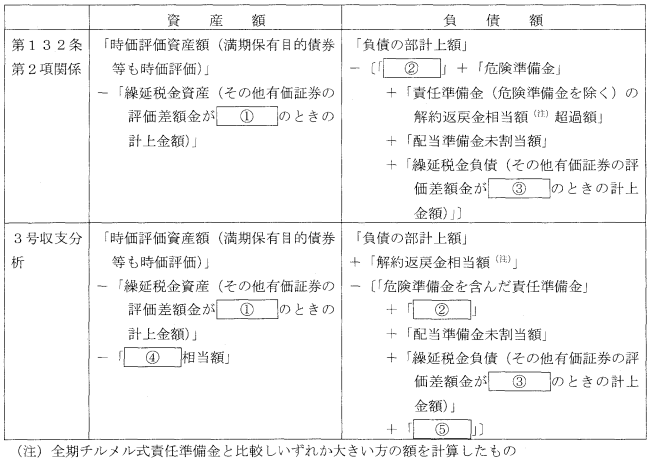
\includegraphics[scale=0.8]{./images/ProbH19-2-1-2.png}

\answer{}
①マイナス②価格変動準備金③プラス④資産運用リスク⑤劣後特約付債務

\problem{H16 生保2問題 1(4)}
事業継続基準の確認に関する保険計理人の実務基準について、次の①〜⑤に入る適切な語句を選
択肢から選び、ア〜タから該当する記号を解答せよ。

事業継続基準の確認の際に「将来の時点における負債の額として合理的な予測に基づき算定され
る額」とは、「第28条に定める事業継続基準に係る額」と「負債の部の合計額から①・価格
変動準備金・配当準備金未割当額・評価差額金に係る繰延税金負債・劣後特約付債務の合計額を
控除した額」の合計額である。

「事業継続基準に係る額」とは、それぞれの保険契約について、②と解約返戻金相当額のい
ずれか大きい方の額を計算したものの合計額である。

第31条第1項の事業継続基準不足相当額は、3号収支分析における分析期間中の最初の③年
間の事業年度末に生じた事業継続基準不足相当額の現価の④とする。

事業継続基準不足相当額が発生した場合に、経営政策の変更によりこの不足相当額が解消される
と保険計理人が判断した場合には、その旨を意見書に示すことができる。この場合の経営政策の
変更とは、資産運用方針の見直し、一部または全部の保険種類の新契約募集の⑤、実現可能
と判断できる事業費の抑制等がある。

〔選択肢〕
ア.3
イ.5
ウ.10
工.20
オ.推進
カ.抑制
キ.最大値
ク.最小値
ケ.合計値
コ.平均値
サ.平準純保険料式責任準備金
シ.5年チルメル式責任準備金
ス、全期チルメル式責任準備金
セ.危険準備金
ソ.貸倒引当金
タ.責任準備金

\answer{}
(4)①タ②ス③イ④キ⑤カ

\section{3号の2収支分析}
\problem{H29 生保2問題 1(3)}
「生命保険会社の保険計理人の実務基準」に定めるソルベンシー・マージン基準の確認に関
する将来収支分析(3号の2収支分析)について、以下の①~⑤の空欄に当てはまる適切な
語句または数値を記入しなさい。

・3号の2収支分析は毎年行うものとし、3号の2収支分析を行う期間(以下「分析期間」とい
う。)は、将来①年間とする。

・3号の2収支分析のシナリオの各要素は、以下に定める通りとする(このシナリオを「3号の
2基本シナリオ」という。)。

 金利は、直近の長期国債応募者利回りが横ばいで推移するものとする。

 株式・不動産の価格や為替レートについては、変動しないものとする。

②の取崩しおよび含み益の実現による積立財源への充当は行わない。

 価格変動準備金・危険準備金等への繰入れは行わない。

 劣後性債務・社債・③
については、その約定に従って、利息を支払うこととする。

保険料積立金等余剰部分控除額の下限は、分析期間中の事業年度末に生じた事業継続基準に係
る額の不足額の④とする。なお、ソルベンシー・マージン比率の算出を行う日におい
て、保険業法施行規則第69条第5項の規定に基づき積み立てた⑤の額を積み立てて
いないものとして計算を行う。

\answer{}
① 5 ② 評価差額金 
③ 基金 
④ 現価の最大値 ⑤ 保険料積立金 

\end{document}